%!TEX root = ../report.tex
\section{Koordination}

\subsection{Begriffe \& Systematik}
\paragraph{Bewegungskoordination meint}
\begin{description}
  \item[Hollmann] das Zusammenwirken von Zentralnervensystem und Skelettmuskulatur innerhalb eines gezielten Bewegungsablaufs
  \item[Starosta] komplizierte Bewegungen genau, schnell und unter verschiedenen Bedingungen durchzuführen
  \item[Mechling] die zeitliche, räumliche und kraftmäßige Steuerung einer Einzelbewegung aufgrund von sensorisch vermittelten Vorgaben
  \item[Neumeier \& Mechling] Bewegungen unter spezifischen Druckbedingen und Informations- anforderungen realisieren
\end{description}
\paragraph{Koordination} Die Fähigkeit, Bewegungen genau und konstant gezielt auszuführen. 
Beispiele: Gleichgewichtssinn, Reaktionsschnelligkeit.
\paragraph{Fähigkeit} eine situations- und zeitabhängige Verhaltensdisposition
\paragraph{Fertigkeit} erpropte, zweckmäßige Bewegungsfolge zur Lösung einer sportlichen Aufgabe
\paragraph{Zusammenhang zwischen Fähigkeiten und Fertigkeiten} Fähigkeiten beinflussen die Ausführung von Fertigkeiten.
Je besser die Fähigkeiten ausgeprägt sind, desto besser ist die Ausführung der Fertigkeit.
Beispiel: Gleichgewichtssinn (Fähigkeit) $\rightarrow$ Handstand, Hechtbagger (Fertigkeit).\\
Kritik: Empirische Analysen liefern für diesen Zusammenhang keine einheitlichen Ergebnisse.\\
Konsequenzen: Begriff der Komponenten der Leistungsfähigkeit anstatt Fähigkeiten als Leistungsvoraussetzungen.
\paragraph{DORFKRUG}
\begin{description}
  \item[D]ifferenzierungsfähigkeit: Kraftdosierung (Ballgefühl, Distanzregulation, \ldots)
  \item[O]rientierungsfähigkeit: räumliche und zeitliche Wahrnehmung und adäquate Reaktion darauf
  \item[R]eaktionsfähigkeit: psychophysische Fähigkeit, auf Reize schnell zu reagieren (c.f. Reaktionsschnelligkeit)
  \item[F] (gibt‘s nicht! „Fähigkeiten“)
  \item[K]opplungsfähigkeit: Teilbewegungen räumlich, zeitlich und dynamisch aufeinander abstimmen.
  \item[R]hythmisierungsfähigkeit: Rythmus von außen erfassen und reproduzieren und inneren Rythmus realisieren
  \item[U]mstellungsfähigkeit: Während einer Handlung Situationsveränderungen wahrnehmen und reagieren.
  \item[G]leichgewichtsfähigkeit: statisch = in Ruhestellung vs dynamisch = in Bewegung/Wiederherstellen des Gleichgewichts
\end{description}
Kritik: alternative Systeme existieren, die sich auch nicht vollständig bewährten.
Für den Leistungssport ist das System der koordinativen Fähigkeiten zu wenig ausdifferenziert $\rightarrow$ eigene Modelle/Begriffe.
\paragraph{Fazit} Das System der koordinativen Fähigekeiten ist wissenschaftlich nicht belegt, aber nützlich fÚr die Taxonomie von Anforderungen und Zielen. 
Steuerung von Bewegungen erfolgt durch fertigkeitsspezifische Qualitäten der Bewegungssteuerung, die trainiert werden können.

\subsection{Determinanten}
\textbf{Koordinationsphänomene und Determinanten}\\
\begin{figure}[H]
  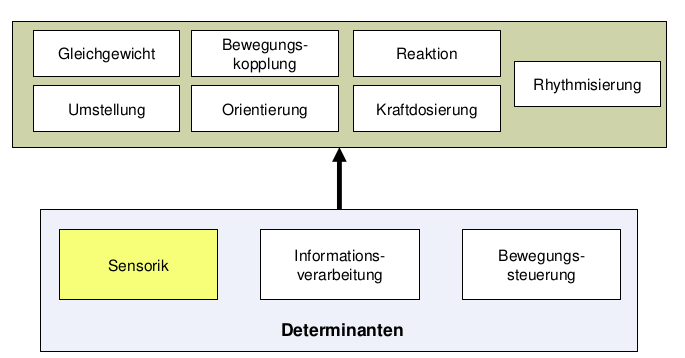
\includegraphics[width=.7\textwidth]{pictures/koordinationsphaenomene_und_determinanten.png}
  \centering
\end{figure}
\paragraph{Sensorik}
\begin{description}
  \item[Visuelles System] Zentrales vs.\ peripheres Sehen, räumliches Sehen, Bewegungssehen (dynamische Sehschärfe, afferent vs efferente Bewegungswahrnehmung)
  \item[Akustisches System]
  \item[Vestibuläres System] Sensorik des Gleichgewichts, befindet sich im Ohr.\\
    Bogengänge: 3-dimensionale Lage-, Bewegungs \& Dreherfassung.\\
    Vorhof: Beschleunigungserfassung.\\
  \item[Somatosensorik] Kälte-/Wärme-, Druck-, Schmerz-, Dehnungs- \& Spannungsrezeptoren.\\
\end{description}
\paragraph{Informationsverarbeitung}
\begin{description}
  \item[Frontaler Cortex] Was ist zu tun?
  \item[Seitlicher Cortex] Wie ist es zu tun?
  \item[Mittlerer frontaler Cortex] Startsignal
\end{description}
\paragraph{Bewegungssteuerung}
\begin{itemize}
  \item Rohbefehl an Motoneurone
  \item Kontrollmitteilung an Kleinhirn
  \item Modulation des Rohbefehls
\end{itemize}
Supraspinalmotorik:
\begin{description}
  \item[Absteigende Bahnen] übermitteln motorische Programme und Aktivieren die Neurosysteme
  \item[Verschaltung mit Motoneuronen] Ausführung der Programme, Monosynaptische Ansteuerung von Motoneuronen durch den Motorcortex um gegen Verschaltungen Abzuschirmen.
  \item[Verschaltung mit Interneuronen] Absteigende Impulse werden durch Interneuronen übertragen.
    Die Bahnen zu geeigneten Muskelgruppen werden entsprechend gewählt.
    Ermöglicht Bewegungskontrolle während der Ausführung.
  \item[Neurone von Rückenmark ins Kleinhirn (aufsteigend)] 
  \item[Neurone vom Rückenmark in höhere Zentren (aufsteigend)] Interneuronale multisensorische Konvergens: Hat die Bewegung das erwartete Resultat gebracht?
\end{description}

\subsection{Trainingsmethoden}
\textbf{Typen von Koordinationstraining}
\begin{figure}[H]
  \centering
  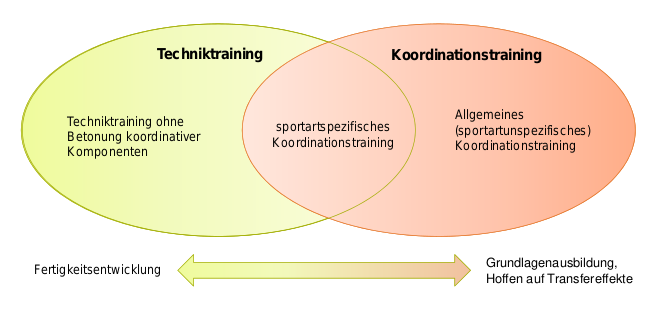
\includegraphics[width=.7\textwidth]{pictures/koordinationstraining_typen.png}
\end{figure}
\paragraph{Belastungsnormative} eher unbedeutend, Inhalte und Durchführung so wählen, dass Wahrnehmung, Informationsverarbeitung und Bewegungssteuerung angesprochen werden.
\paragraph{Koordinationsübung} = beherrschte Fertigkeiten (Laufen, Pritschen,\ldots) + Informationsverarbeitung und Bewegungssteuerung (Präzisions-, Zeit-, Komplexitäts-, Belastungs- und Variabilitätsdruck) + unterschiedliche Sensorik (optisch, akustisch, \ldots)

\subsection{Trainingsinhalte}

\subsection{Anwendung}

\subsection{Diagnostik}
